%% Преамбула TeX-файла

% 1. Стиль и язык
\documentclass[utf8x, 14pt]{G7-32} % Стиль (по умолчанию будет 14pt)

% Остальные стандартные настройки убраны в preamble.inc.tex.
\sloppy

% Настройки стиля ГОСТ 7-32

% Добавляем гипертекстовое оглавление в PDF
\usepackage[
bookmarks=true, colorlinks=true, unicode=true,
urlcolor=black,linkcolor=black, anchorcolor=black,
citecolor=black, menucolor=black, filecolor=black, urlcolor=blue,
]{hyperref}
\AfterHyperrefFix

\usepackage{microtype}% пакет для микротипографии, под pdflatex хорошо улучшает читаемость

% Тире могут быть невидимы в Adobe Reader
\ifInvisibleDashes
\MakeDashesBold
\fi

\usepackage{graphicx}   % Пакет для включения рисунков
\usepackage{tikz}
\graphicspath{ {./images/} }

\geometry{right=20mm}
\geometry{left=30mm}
\geometry{bottom=20mm}
\geometry{ignorefoot}


\setlength{\parskip}{1ex} % разрыв между абзацами

% Упрощение написания ссылки
\newcommand\case[1]{По Случаю #1 из Теоремы 2.6 из \cite{hse:Teoria_Gener}}





% Стиль титульного листа и заголовки
% Титульная страница, по умолчанию ГОСТ 7.32-2001,  
 
\NirOrgLongName{Правительство Российской Федерации\par
Федеральное государственное автономное образовательное\\
учреждение высшего образования\\
"Национальный исследовательский университет\\
"Высшая школа экономики"\\
Московский институт электроники и математики им. А.Н. Тихонова\\
Департамент прикладной математики
} 


\NirReportName{Методические материалы}
\NirAbout{По дисциплине \par "Теория псевдослучайных генераторов"} 


\Nir{Разбор практических задач с теоретическим обоснованием}

\NirSubject{Типовые задачи контрольных работ}                                
\NirCode{}

\NirManager{Преподаватель дисциплины}{М.И. Рожков }
\NirIsp{Руководитель создания документа}{А.Ю. Нестеренко}

\NirYear{2021}
\NirTown{Москва}



\begin{document}

\frontmatter % выключает нумерацию; здесь начинаются НЕнумерованные главы: введение, глоссарий, сокращения.

\maketitle % создает титульную страницу


\begin{executors}
\personalSignature{Выполнил студент}{Щеглова П.Н.}
\end{executors}

\tableofcontents % создает содержание документа
 

\Introduction

Целью работы является демонстрация навыков подготовки электронных документов в системе компьютерной верстки документов latex. Выполнены требования к подготавливаемому документу:

\begin{itemize}
\item титульный лист по ГОСТ 7.32-2001;
\item общий объем документа не менее 18 страниц;
\item наличие разделов документа, включая ненумерованные (введение, обозначения и т.п.);
\item наличие формул (строчные и выключенные);
\item наличие ссылок (по документу и внешних);
\item наличие таблиц, изображений и т.п.;
\item наличие списка литературы и ссылок на него по тексту документа;
\item определение собственных команд, упрощающих процесс набора документа;
\item отсутствие орфографических ошибок, наличие смысла в подготовленном документе,
обоснование, для чего документ подготовлен;
\item краткая информация о сборке документа и используемых шрифтах, размерах (шрифтов, полей и т.п.);
\item информация о том, какие стилевые пакеты применяли и для какой цели.
\end{itemize}

Содержательно документ подготовлен для демонстрации студентам, проходящим курс теории псевдослучайных генераторов, хода решения типовых задач из контрольноых работ, для некоторых типов задач приведено решение для всех вариантов входных параметров. Первыми разбираются общие задачи для двух контрольных, затем уникальные для первой контрольной задачи и для второй. Теоретические обоснования даны в виде ссылок на соответствующие утверждения из источников и частично продублированы в виде утверждений. 
 % создает раздел Введение


\mainmatter % это включает нумерацию глав и секций в документе ниже

\chapter{Шифрование с сохранением формата}

\section{Описание концепции}
Format-preserving encryption, сокращенно FPE, - тип шифрования, который подразумевает сохранение формата открытого текста в шифртексте, или более формально отображение из множества открытых текстов в то же самое множество. Примеры отображений: шифрование 16-значного номера банковской карты 16-значным числом; шифрование одного английского слова другим английским словом; шифрование n-битного числа n-битным числом (совпадает с определением n-битного блочного шифра).


Для конечных множеств данный тип шифрования эквивалентен перестановке перенумерованных элементов множества. Истинно случайная перестановка является идеальным шифром FPE, однако для больших множеств невозможно предварительно сгенерировать и запомнить такую перестановку. Таким образом, проблема FPE состоит в том, чтобы сгенерировать псевдослучайную перестановку из секретного ключа таким образом, чтобы время вычисления для одного значения было небольшим (в идеале постоянным, но, что наиболее важно, меньшим, чем $O(N)$, где $N$ - размер входных данных).


Алгоритм FPE можно реализовать с использованием сети Фейстеля. Сеть Фейстеля нуждается в источнике псевдослучайных значений для раундовых ключей, выходные данные алгоритма AES могут использоваться в качестве этих псевдослучайных значений. 


Чтобы реализовать алгоритм FPE с использованием AES и сети Фейстеля, можно использовать столько битов вывода AES, сколько необходимо, чтобы получить последовательность с длиной равной длине левой или правой половины сети Фейстеля. Если, например, в качестве раундового ключа требуется 24-битное значение, можно использовать 24 младших бита вывода AES.


При данном подходе выходные данные сети Фейстеля не обязательно сохранят формат входных данных, поэтому итерации сети Фейстеля повторяются с помощью cycle-walking до тех пор пока формат не совпадет. Поскольку размер входов в сеть Фейстеля настраеваем, можно сделать наиболее вероятным, что эта итерация завершится в среднем достаточно быстро. В случае номеров кредитных карт, например, существует $10^{15}$ возможных 16-значных номеров кредитных карт (с учетом избыточной контрольной цифры), а поскольку $10^{15} \approx 2^{49,8}$, с использованием 50-битной сети Фейстеля и cycle-walking можно создать алгоритм FPE, который в среднем зашифровывает довольно быстро.

\section{Действующие стандарты} % Добавить ссылки на стандарты
Существует множество реализованных алгоритмов типа FPE, к актуальным можно отнести разработанные в США FF1 и FF3-1, а также южно-корейские FEA-1 и FEA-2.
Алгоритм FEA, представленный институтом исследований национальной безопасности (NSR), использует сети Фейстеля, аналогичные стандартам NIST, FF1 и FF3-1. Однако алгоритмы FF1 и FF3-1 используют блочные шифры как F-функции, в то время как FEA использует свои собственные специализированные функции. Эта особенность позволяет использовать более высокоскоростное шифрование по сравнению с другими алгоритмами, предназначенными для шифрования с сохранением формата. FEA может быть подходящим выбором, при шифровании конфиденциальной персональной информации, которая, как правило, имеет небольшой объем.


Разница между этими двумя алгоритмами состоит в том, что FEA-1 имеет размер настройки $128-n$ бит (где $n$ - размер входной последовательности), каждый с 12, 14 и 16 раундами при длине двоичного ключа 128, 192 и 256 соответственно. FEA-2 имеет фиксированный размер параметра настройки в 128 бит с 18, 21 и 24 раундами при длинах ключей 128, 192 и 256 соответственно.

\subsection{FEA-1}
Опишем подробнее стандарт, который анализируется в данной работе, а именно FEA-1:

\begin{figure}[h!]
	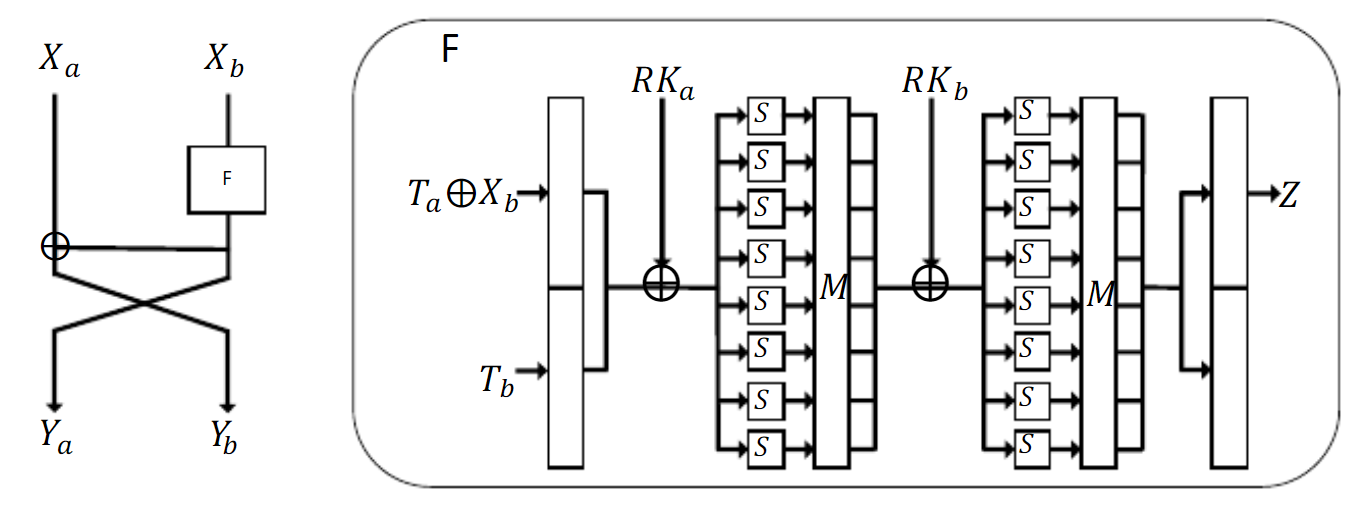
\includegraphics[width = \textwidth]{FEA-1 structure.png}
	\caption{Структура итерации FEA, на основе сети Фейстеля}
	\label{fig:fea_structure}
\end{figure}

На вход алгоритму подаются последовательности чисел из конечного множества, мощностью от $2^8$ до $2^{128}$, размер двоичного ключа $K$ составляет $\in [ 128, 192, 256 ]$. Алгоритм представляет собой последовательное применение итераций сети Фейстеля, ее общая схема представлена в левой части Рисунка \ref{fig:fea_structure}. Входная последовательность итерации $X$ делится на две равные части $X_a$ и $ X_b$, $X_b$ передается на вход специализированной $F$-функции, общая схема которой обозначена в правой части Рисунка \ref{fig:fea_structure}. $T_a$ и $T_b$ - левая и правая половины нстройки, принцип формирования которой будет описан далее, $RK_a$ и $RK_b$ - левая и правая половины раундового ключа, $S$ - блок подстановки (в данной схеме применяются идентичные $S$-блоки), $\mathcal{M}$ - блок умножения на заданную матрицу.


Выбор настройки для каждой итерации происходит по следующему алгоритму: настройка $T$ (битовый вектор длины $128-n$) делится на две под-настройки $T_L = T_{ [ 0:64-n_2-1 ] }$ и $T_R=T_{ [ 64-n_2:128-n-1 ] }$ длины $64-n_2$ и $64-n_1$, соответственно. Полагаем $T_a^i=0$ для каждой итерации и $T_b^i$ для $i$-ой итерации, как:

$$ T_b^i =
\begin{cases}
T_L & \dfrac{i}{2} \in N \\
T_R & \dfrac{i+1}{2} \in N
\end{cases} $$

\section{Линейный метод}

Линейный метод криптографического анализа состоит из двух этапов: 
\begin{enumerate}
    \item Нахождение линейного статистического аналога для части исходного блочного шифра, это линейное соотношение связывает входные и выходные значения выбранной части алгоритма. Оно должно выполняться с вероятностью заметно отличающейся от случайной для возможности отличения этих двух вариантов событий.
    \item Отбрасывание ложных ключей с использованием найденного вероятностного соотношения.
\end{enumerate}

\begin{figure}[h!]
	\centering
	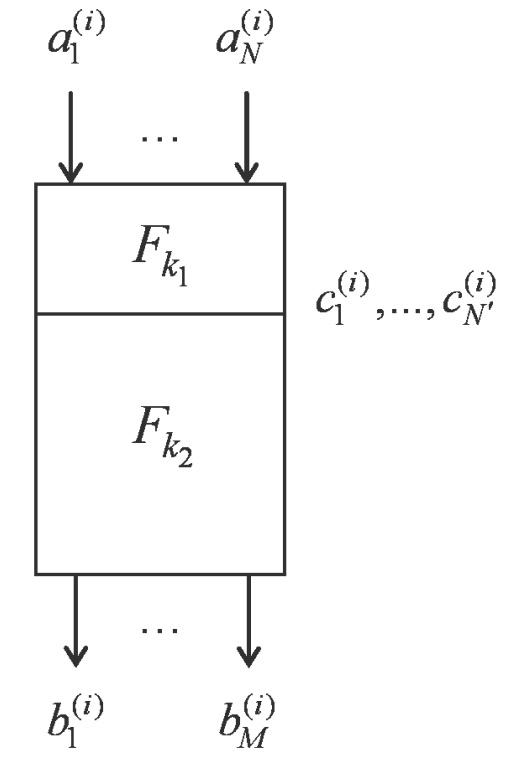
\includegraphics[scale=0.25]{linan.png}
	\caption{Схема разбиения алгоритма на два блока для проведения линейного криптографического анализа}
	\label{fig:linan}
\end{figure}

Перейдем к описанию метода:

Пусть схема шифропреобразования с общим ключом $K$ разбита на две последовательные части $F_{K_1}$ и $F_{K_2}$, как показано на Рисунке \ref{fig:linan}. В первой из них используется небольшая часть исходного ключа $K_1$, во второй, соответсвенно, большая $K_2$ (при этом $K_1$ может частично совпадать с $K_2$). Пусть также найдено линейное соотношение 
\begin{equation}
\label{eqn:eq1}
c_1^{(i)} L_1^{'} + ... + c_N^{(i)} L_N^{'} \backsimeq b_1^{(i)} L_1^{''} + ... + b_N^{(i)} L_N^{''} ,\end{equation}
 которое, \textbf{независимо от значения $K_2$}, выполняется с вероятностью $P = \dfrac{1+\delta}{2}$, где $\delta \neq 0$.

Булевы величины $L_j^{'}$ и $L_s^{''}$, $j,s \in \overline{1,N}$(маска найденного линейного соотношения) известны; $c_1^{(i)}, ..., c_N^{(i)}$  - промежуточный шифртекст, между двумя блоками шифропреобрахования; $b_1^{(i)}, ..., b_N^{(i)}$ - известный итоговый шифртекст, $a_1^{(i)}, ..., a_N^{(i)}$ - известный открытый текст, $i \in \overline{1,T}$, где $T$ - количество материала.

Пусть $K_1^{'}$ - доля ключа $K_1$, от которой зависит левая часть в соотношении \ref{eqn:eq1}. Если при опробовании $K_1^{'}$ выполнимость соотношения с вероятностью $P = \dfrac{1+\delta}{2}$ не подтверждается, то соответствующее значение $K_1^{'}$ отбраковывается. Чем больше при этом $T$ и $|\delta|$, тем большая доля значений $K_1^{'}$ будет отбракована, вплоть до однозначного определения $K_1^{'}$.


\subsection{Их идеи}
Линейный криптоанализ основан на вероятностных линейных соотношениях или линейных приближениях. Пусть $F: \mathbb{F}_2^n \to \mathbb{F}_2^m$ - функция, возможно зависящая от ключа. Линейные различители строятся на основе линейных приближений с большой абсолютной корреляцией. Линейное приближение для $F$ определяется двумя масками $(u_1,u_2) \in \mathbb{F}_2^n \oplus \mathbb{F}_2^m$, и их корреляция равна:
$$ C_{u_1,u_2}^F = 2\cdot P\left(u_1^\top F(x) = u_2^\top x\right)-1 = \dfrac{1}{2^n} \sum_{x\in F_2^n} (-1)^{u_1^\top F(x) + u_2^\top x},$$
где вероятность считается от равновероятно распределенного $x\in \mathbb{F}_2^n$. Если $u_1 \neq 0$, то математическое ожидание корреляции равновероятно распределенной функции равно нулю, а стандартное отклонение $\sigma = 2^{-n/2}$. Следовательно, если корреляция $C$ значительно превосходит $2^{-n/2}$, то различителем можно считать вычисление корреляции для $q=\Theta (1/c^2)$ пар масок и сравнение получившего значения с некоторым заданным пороговым значением.

На первый взгляд стандарты FEA-1 и FEA-2 кажутся стойкими к линейному криптоанализу, особенно когда их раундовые функции F заменены на равновероятные случайные функции. Основное замечение, которое можно эксплуатировать в атаках на такие шифры, состоит в том, что шифр оказывается нестойким, если настройка (его часть) считается частью входных данных.

\begin{figure}[h!]
	\centering
	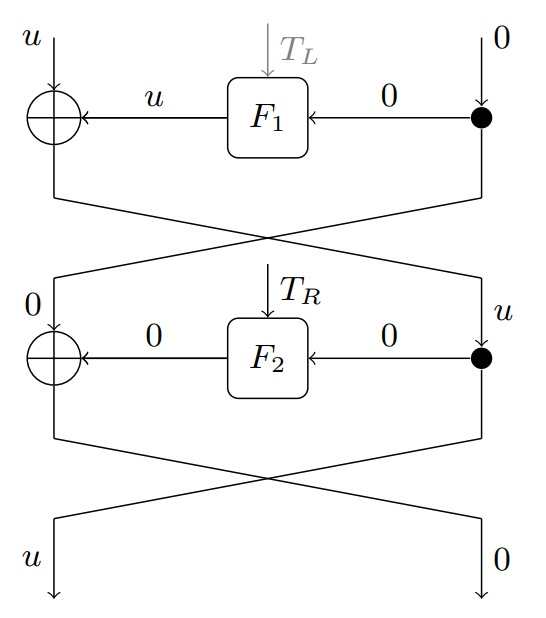
\includegraphics[scale=0.5]{trial.png}
	\caption{Две итерации FEA-1}
	\label{fig:trial}
\end{figure}

Рассмотрим испытание двух итераций FEA-1 (Рисунок \ref{fig:trial}), настройка $T_L$ - произвольная постоянная, а $T_R$ считается переменной входа. Если это не так, то для проведения атаки $T_R$ должна быть известной. Идея состоит в том, что абсолютная корреляция линейного приближения раундовой функции $F_i$ превышает $1/\sqrt{N} = 2^{-m/2}$ с достаточно большой вероятностью, что важно, когда настройка включается во входные данные, потому что область определения функции, которая отображает настройку и открытый текст в шифртекст, велика. В самом деле, математическое ожидание корреляции линейных приближений над случайной функцией с тем же размером входа (включая $T_R$ размера $64-m$), что и в FEA-1, равно нулю,а стандартное отклонение $2^{-32-m/2}$. 

\subsubsection{Теорема}\label{theorem}

 Пусть $C$ - корреляция нетривиального линейного приближения равновероятно распределенной функции $F: \mathbb{F}_2^n \to \mathbb{F}_2^m$. Случайная величина $2^{n-1}(C+1)$ имеет биномиальное распределение с математическим ожиданием $2^{n-1}$ и дисперсией $2^{n-2}$. В частности, при $n\to\infty$ распределение $2^{n/2}C$ сходится к стандартному нормальному распределению $\mathcal{N}(0,1)$.

\subsubsection{Применение}

Пусть $r\leq 2$ - четное целое число. По принципу набегания знаков, корреляция испытания $r$ раундов равна $C=\prod_{i=1}^{r/2} C_i$, где $C_i \thicksim \mathcal{N}(0,1/N)$ по Теореме \ref{theorem}. Случайные переменнные $C_i$ будем считать независимыми, что следует из предположения о независимости раундовых функций $F_1, F_3, ..., F_{r-1}$. Можно проверить, что другие испытания для FEA-1 имеют коррелицию пренебрежимо малую.

Как упоминалось ранее, объем материала (или степень нелинейности???) для линейного различителя, основанного на приближении, с корреляцией $C$ равен $\Theta (1/C^2)$. В таком случае, значение корреляция сильно варьируется в зависимости от ключа, поэтому полученный результат нельзя напрямую использовать для вычисления объема материала. Эвристически вычислимо, что для FEA-1
\begin{equation}
\label{eqn:keyeq}
1/\mathbb{E}(c^2)=N^{r/2},\end{equation} 
где $\mathbb{E}(c^2)$ - средне-квадратичная корреляция для равномерно распределенного случайного ключа. При этом, если правая часть открытого текста фиксирована проивользной константой, то после двух раундов левая половина промежуточного шифртекста равна левой половине открытого текста с точностью до константы. Следовательно, первые два раунда можно эффективно пропустить. Такая возможность, уменьшает степень нелинейности выхода в $N$ раз до $N^{r/2-1}$.



% \cite{hse:Teoria_Gener} любой характеристический многочлен ЛРП кратен минимальному многочлену. Тогда достаточно проверить делители характеристической функции.





\backmatter %% Здесь заканчивается нумерованная часть документа и начинаются ссылки

% % Список литературы при помощи BibTeX
% Юзать так:
%
% pdflatex main
% bibtex main
% pdflatex main

\bibliographystyle{ugost2008}
\bibliography{main}

%%% Local Variables: 
%%% mode: latex
%%% TeX-master: "main"
%%% End: 



%\appendix   % Тут идут приложения

%\include{90-appendix1}

%\include{91-appendix2}

\end{document}

%%% Local Variables:
%%% mode: latex
%%% TeX-master: t
%%% End:
